\documentclass{article}
\usepackage{epsfig}
\usepackage{graphicx}
%\usepackage[a4paper, total={6in, 10in}]{geometry}
\usepackage[table]{xcolor}
\usepackage{tikz}
\title{CS345 Programming Assignment 1 \\ }
\author{\vspace{2mm} \large Ayush Agarwal, 13180 \\ M.Arunothia, 13378}
\date{}
\begin{document}
\maketitle
\section{Red-Blue line segments}
\subsection{Algorithmic Description}
For the given $2*n$ line segments ($n$ vertical red and $n$ horizontal blue) (inside the square defined by (0,0) and (1,1))  our implementation does the following to find the number of intersection. \\*
\begin{itemize}
\item We use a line sweep along the Y-direction.
\begin{center}
\begin{tikzpicture}
\draw[step=1cm,gray,very thin] (-2,-2) grid (6,6);
\filldraw[fill=white, draw=black] (-2,-2) rectangle (6,6);
\draw[green,thick,dashed] (-2,0) -- (6,0);
\draw[blue,thick] (0,0) -- (2,0);
\draw[blue,thick] (3,3) -- (5.5,3);
\draw[blue,thick] (1.5,-1.5) -- (4,-1.5);
\draw[blue,thick] (-1.8,2) -- (2,2);
\draw[red,thick] (1,-0.5) -- (1,4);
\draw[red,thick] (-1,3) -- (-1,5.5);
\draw[red,thick] (4,1.7) -- (4,5.8);
\draw[red,thick] (2.7,0) -- (2.7,5);
\node [yellow] at (2.7,0) {\textbullet};
\node [yellow] at (1,-0.5) {\textbullet};
\node [yellow] at (-1,3) {\textbullet};
\node [yellow] at (4,1.7) {\textbullet};
\node [violet] at (2.7,5) {\textbullet};
\node [violet] at (1,4) {\textbullet};
\node [violet] at (-1,5.5) {\textbullet};
\node [violet] at (4,5.8) {\textbullet};
\node [violet] at (2.7,5) {\textbullet};
\end{tikzpicture}
\end{center}
\item The green dashed line in the above figure shows our sweep line. This basically means that the horizontal blue lines are processed in increasing $y$ co-ordinates.
\item All yellow points (bottom point of red lines) that lies below or on the sweep line indicate those red lines that can potentially cause an intersection with the blue line. So, the $x$-coordinates of these yellow points are inserted into the BST maintained.
\item All violet points (top point of red lines) that lies above the sweep line indicate those red lines that can no longer cause an intersection with the blue line. So, the $x$-coordinates of these violet points are deleted from the BST maintained.
\item Now the number of intersections of this blue line (say is defined by $(x_1,y),(x_2,y)$)  are found by finding the number of nodes in the BST having $x$ in the range $[x_1,x_2]$.
\item To optimize the above implementation, the BST was augmented by sub-tree size along with usual node data.
\item Two implementations of the range count was done, with first one being submitted -
\begin{itemize}
\item By finding count of $x > x_2$ and $x >= x_1$ and by taking their difference for the required range. 
\item by LCA method
\end{itemize} 
\end{itemize}
\subsection{Implementation Description}
\begin{itemize}
\item {\bf Language of Implementation} - C++ 
\item {\bf Number of lines of Code} - 190 lines (including time and random generator functions)\\*
\item {\bf Configuration of System used for Experiment}
\begin{center}
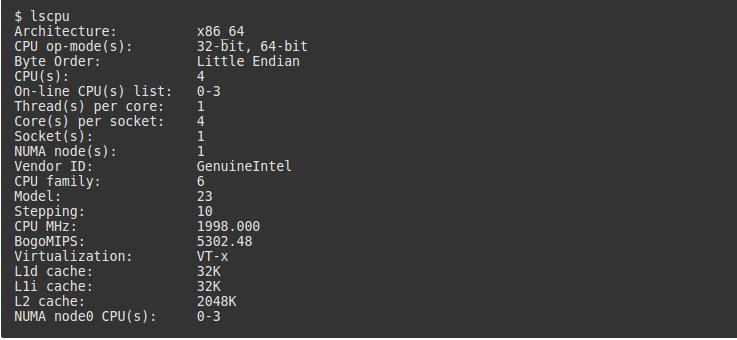
\includegraphics[scale=0.5]{system_conf.png}
\end{center}
\item {\bf Number of repetitions} made for a given {\bf $n$} is {\bf $10^7/n$}. 
\item {\bf Range of $n$ } is {\bf $\{1,10,10^2, 10^3, 10^4, 10^5, 10^6, 10^7 \} $}
\end{itemize}
\hspace*{-2.5cm}\begin{tabular}{|p{1cm}|p{2.5cm}|p{2.5cm}|p{1.5cm}|p{1.5cm}|p{4cm}|}
 \hline
 \multicolumn{6}{|c|}{Result Table} \\
 \hline
 $n$   & Time(seconds) & No. of Intersections & $n^2/9$ &  $n *\log n $ & $(10^7 * Time/n* \log n)$\\
 \hline 
 $1$   	& $0$ 		& $0.1111$	& $ $ 	& $ $  	& $ $	\\
 \hline
 $10$  	& $4.00E-06$	& $11.1052$ & $ $	& $ $	& $ $	\\
 \hline
 $10^2$	& $7.00E-05$	& $1110.92$	& $ $	& $ $	& $ $	\\
 \hline
 $10^3$	& $0.0011$	& $111082$	&  	&	&	\\
 \hline
 $10^4$	& $0.015$  	& $1.11E+07$	&	&	&	\\
 \hline
 $10^5$	& $0.25$ 	& $1.11E+09$&	&	&	\\
 \hline
 $10^6$	& $4.8$		& $1.11E+11$&	&	&	\\
 \hline
 $10^7$	& $62$		& $1.11E+13$&	&	&	\\
 \hline
\end{tabular}
\end{document}
